\section[KG-based IR]{KG-based Information Retrieval}

\begin{frame}{Experiments objective}

    % \begin{center}
    %     From a text-based to a concept-based search.
    % \end{center}

    \begin{figure} [H]
        \begin{center}
            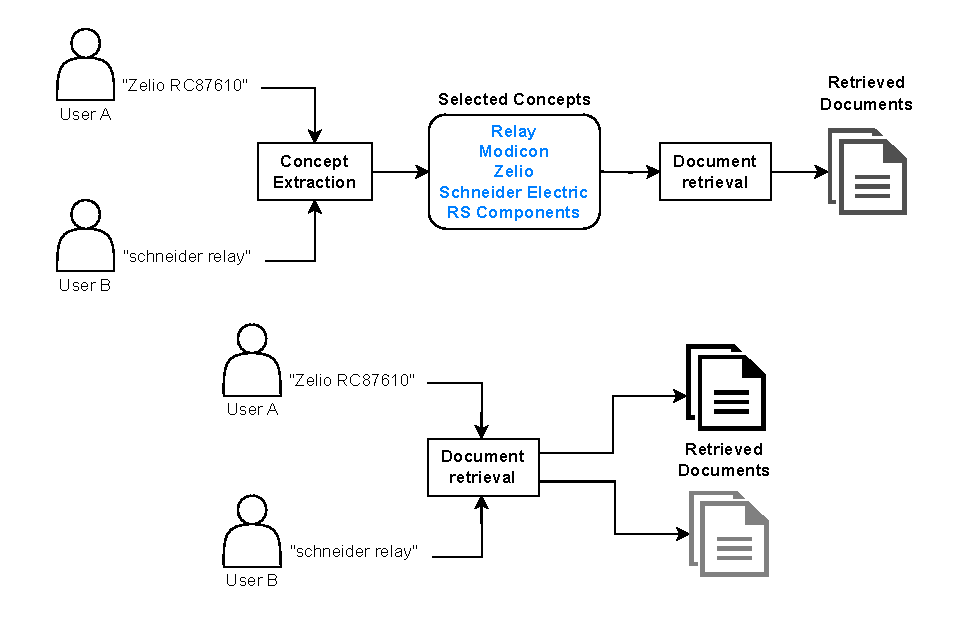
\includegraphics[scale=0.6]{images/text-vs-concept-based-search.pdf} 
            \caption{Text-based vs concept-based search.} 
        \end{center}
    \end{figure}

\end{frame}

\begin{frame}{Evaluation metrics}

    \begin{itemize}
        \item Mean Average Precision at k (MAP@k): 
        \begin{itemize}
            \item A sliding (or growing) precision window, averaged over a set of query examples.
            \item Ranges from $0$ to $1$ ($1$ is the best value).
            \item Gives information about the amount and positions of positive results in the k first ones.
        \end{itemize}
        \item Binary Mean at k (BM@k):
        \begin{itemize}
            \item Binary average over a set of query examples.
            \item Ranges from $0$ to $1$ ($1$ is the best value).
            \item Provides information about the amount of queries with a positive result in the k first ones.
            \item Does not give any detail on the positive result position.
        \end{itemize}
    \end{itemize}

\end{frame}